\documentclass[12pt,a4paper]{article}

\usepackage[utf8]{inputenc}
\usepackage[T1]{fontenc}
\usepackage[english]{babel}
\usepackage{graphicx}
\usepackage{float}
\usepackage{geometry}
\usepackage{hyperref}
\usepackage{enumitem}
\usepackage{lmodern}
\usepackage{microtype}
\usepackage{needspace}
\usepackage[font=small,labelfont=bf]{caption}
\usepackage{array,tabularx}
\usepackage{pdflscape}

\setlength{\parindent}{0pt}
\setlength{\parskip}{0.4em}
\raggedbottom
\newcommand{\storyfront}[5]{%
  \par\noindent\fbox{%
    \begin{minipage}{\dimexpr\linewidth-2\fboxsep-2\fboxrule\relax}
      \small
      \textbf{ID: #1}\hfill\textbf{TITLE: #2}\par\smallskip
      \begin{tabularx}{\linewidth}{@{}>{\raggedright\arraybackslash}p{0.15\linewidth}|>{\raggedright\arraybackslash}X|>{\raggedright\arraybackslash}X@{}}
        \textbf{As a/n\ldots} & \textbf{I want to\ldots} & \textbf{so that I can\ldots} \\
        \hline
        #3 & #4 & #5
      \end{tabularx}
    \end{minipage}%
  }\par
}
\newsavebox{\storycardbox}
\newenvironment{storyback}{%
  \par\begin{lrbox}{\storycardbox}%
  \begin{minipage}{\dimexpr\linewidth-2\fboxsep-2\fboxrule\relax}
  \small
  \setlist[itemize]{leftmargin=1.5em,itemsep=0.35em,topsep=0.4em,parsep=0pt}
}{%
  \end{minipage}\end{lrbox}%
  \noindent\fbox{\usebox{\storycardbox}}\par
}

\setlength{\parindent}{0pt}
\setlength{\parskip}{0.4em}
\raggedbottom
\setlist[enumerate]{itemsep=0.35em,topsep=0.4em}
%%jak cos ten slop jest po to zeby te diagramy jakkolwiek sensowne byly
\usepackage{tikz}
\usetikzlibrary{arrows.meta,shapes.geometric,shapes.multipart}
\definecolor{ink}{HTML}{213547}
\definecolor{accent}{HTML}{245B78}
\definecolor{soft}{HTML}{F4F8FB}
\definecolor{muted}{HTML}{536675}
\tikzset{
  boundary/.style={draw=ink!65,rounded corners=3mm,line width=.7pt,fill=soft},
  usecase/.style={ellipse,draw=accent,line width=.8pt,fill=white,
    align=center,text=ink,font=\small,minimum width=7.5cm,
    minimum height=1.3cm,text width=5.8cm,inner sep=2pt},
  association/.style={draw=ink!75,line width=.65pt},
  include/.style={dashed,-{Stealth[length=2mm]},draw=ink,line width=.7pt},
  note/.style={draw=ink!35,rounded corners=2mm,fill=white,
    text=muted,font=\small,align=left,inner sep=3mm}
}
\newcommand{\umlactor}[4]{%
  \begin{scope}[shift={(#2,#3)},draw=ink,line width=.8pt]
    \draw (0,.45) circle (.18);
    \draw (0,.27)--(0,-.35);
    \draw (-.34,.03)--(.34,.03);
    \draw (0,-.35)--(-.30,-.82);
    \draw (0,-.35)--(.30,-.82);
    \coordinate (#1) at (.34,.03);
    \coordinate (#1-top) at (0,.66);
    \coordinate (#1-bottom) at (0,-.84);
    \node[below,text=ink,font=\small,align=center] at (0,-.9) {#4};
  \end{scope}
}
\tikzset{
  umlclass/.style={rectangle split,rectangle split parts=2,
    rectangle split part align={center,left},
    rectangle split part fill={soft,white},draw=accent,line width=.65pt,
    text=ink,text width=4.25cm,inner sep=4pt,font=\footnotesize},
  umlrelation/.style={draw=ink!85,line width=.65pt},
  umldependency/.style={draw=ink!85,dashed,-{Straight Barb[length=2mm]},
    line width=.65pt},
  umlrealisation/.style={draw=ink!85,dashed,
    -{Triangle[open,length=2.8mm,width=2.8mm]},line width=.65pt},
  umlmultiplicity/.style={font=\scriptsize,text=ink,fill=white,
    inner sep=1.2pt},
  umlcaption/.style={font=\scriptsize,text=muted,fill=white,
    inner sep=1.5pt,align=center}
}
\newcommand{\storyref}[1]{{\scriptsize\color{muted}#1}}


\geometry{margin=2.5cm}

\usepackage{titlesec}

\titlespacing*{\section}{0pt}{2.5ex}{1ex}
\titlespacing*{\subsection}{0pt}{2ex}{0.8ex}

\titleformat{\subsubsection}
  {\normalfont\normalsize\bfseries}
  {}{0pt}{}

\titlespacing*{\subsubsection}
  {0pt}{2.5ex}{0.6ex}

  
\titleformat{\subsection}
  {\normalfont\large\bfseries}
  {\thesubsection}{1em}{}
  [\titlerule]


\title{\textbf{NarrativeWatch} Checkpoint 1}

\author{
    Karolina Małaśnicka \\
    Maciej Majewski \\
    Mateusz Wietecki \\
    Kacper Frączek \\
    Jan Czyżewski
}

\date{October 2026}

\begin{document}

\maketitle
\vspace{-1.5cm}
\tableofcontents
\newpage

\section{Project Overview}

\subsection{Project Description}
NarrativeWatch is a system designed to monitor, detect and analyze foreign information manipulation and interference (FIMI) narratives in online articles and posts. The application collects content from selected sources and uses AI agents to find matches with known FIMI narratives. An LLM Judge checks these matches and provides explanations and confidence scores, while human analysts review uncertain cases. The goal is to detect potentially manipulative narratives before they spread widely.

\subsection{Main Features \& Architecture}
NarrativeWatch consists of several components that work together to collect, analyze and verify online content.

\begin{enumerate}
    \item \textbf{Crawler Agent:} Collects new articles and posts from monitored sources on a schedule.
    \item \textbf{Analysis Agent:} Analyzes collected content and matches it with known FIMI narratives.
    \item \textbf{LLM Judge Agent:} Verifies potential matches and provides explanations and confidence scores.
    \item \textbf{API Server:} Provides a REST API and handles authentication, user roles and data storage.
    \item \textbf{Analyst Dashboard:} Allows analysts to view detected narratives and alerts, and review uncertain matches.
    \item \textbf{Admin Panel:} Allows administrators to manage monitored sources and the database of known narratives.
\end{enumerate}




\section{User Stories}

The following user stories describe the main functionalities of NarrativeWatch from the perspective of its users. The main user roles are Analyst and Admin.

\subsection{Analyst User Stories}
\subsubsection*{US-01 -- View Detected Narratives}
As an analyst, I want to view detected FIMI narratives so that I can monitor possible disinformation.

\subsubsection*{US-02 -- View Alerts}
As an analyst, I want to see alerts about suspicious content so that I can quickly identify articles that may need attention.

\subsubsection*{US-03 -- View Article Details}
As an analyst, I want to view the content and source of an article that potentially matches a known FIMI narrative so that I can better understand its context.

\subsubsection*{US-04 -- View Narrative Matches}
As an analyst, I want to see which known narratives an article matches so that I can understand why it was flagged.

\subsubsection*{US-05 -- View LLM Judge Results}
As an analyst, I want to see the LLM Judge's decision, explanation and confidence score so that I can understand how the match was evaluated.

\subsubsection*{US-06 -- Review Uncertain Matches}
As an analyst, I want to review matches with low confidence scores so that I can decide whether they are correct.

\subsubsection*{US-07 -- Save Review Decisions}
As an analyst, I want my review decisions to be saved so that they can be used as ground truth for evaluating the LLM Judge.

\subsubsection*{US-08 -- View Narrative Trends}
As an analyst, I want to view trends in detected narratives so that I can see how frequently they appear in monitored content.

\subsubsection*{US-09 -- Propose a New Narrative}
As an analyst, I want to propose a new narrative linked to a content item
so that previously unknown narratives can be considered for inclusion
in the shared catalogue.

\subsubsection*{US-10 -- Review Narrative Proposals}
As an analyst, I want to review and approve or reject narratives proposed
by other analysts so that the shared catalogue contains verified narratives.

\subsubsection*{US-11 -- Track Narrative Proposal Status}
As an analyst, I want to see the status and review decisions for my narrative
proposals so that I know whether they are awaiting review, approved or rejected.

\subsubsection*{US-12 -- View Analysis Results}


As an analyst, I want collected articles to be automatically analyzed and potential narrative matches to be verified by the LLM Judge so that I can review the results without checking every article manually.

\subsection{Admin User Stories}

\subsubsection*{US-13 -- Add Monitored Sources}
As an admin, I want to add sources to monitor so that the system can collect articles and posts from them.

\subsubsection*{US-14 -- Manage Monitored Sources}

As an admin, I want to edit or remove monitored sources so that the system only collects content from relevant sources.

\subsubsection*{US-15 -- Manage Known Narratives}

As an admin, I want to update or remove existing narratives so that the narrative database stays up to date.

\subsubsection* {US-16 -- View Reviewer Activity}
As an admin, I want to view each reviewer's match decisions, narrative proposals
and proposal reviews so that I can oversee the review process.

\subsubsection*{US-17 -- Add Known Narratives}

As an admin, I want to add new FIMI narratives to the database so that the system can detect them in collected content.

\subsection{General User Stories}

\subsubsection*{US-18 -- Log Out}
As a user, I want to log out of the application so that I can securely end my session.

\subsubsection*{US-19 -- Access Features Based on Role}
As a user, I want to access only the features assigned to my role so that I can use the application with the appropriate permissions.

\subsubsection*{US-20 -- Log In}
As a user, I want to log in to the application so that I can access the features available to my role.

\clearpage




\section{Detailed User Stories}
The crucial requirements are specified as user story cards. Each front side
states the role, feature and business justification. Each reverse side gives
functional acceptance criteria and non-functional requirements as yes/no
questions. The UC identifiers refer to the diagrams in
Section~\ref{sec:use-case-diagrams}.

\subsection{US-05 -- View LLM Judge Results}
\textbf{Related use case:} UC-A1 (Explore analysis results).

\begin{figure}[H]
\setlength{\fboxsep}{7pt}
\storyfront{US-05}{View LLM Judge Results}
  {Analyst}
  {see the LLM Judge's decision, explanation and confidence score}
  {understand how the match was evaluated.}
\caption{Front side of the US-05 user story card.}
\end{figure}

\begin{figure}[H]
\setlength{\fboxsep}{7pt}
\begin{storyback}
\textbf{Acceptance criteria checklist}\\
(Functionality)
\begin{itemize}
  \item Can I view the Judge's decision, explanation and confidence score
        for a selected narrative match?
  \item Can I identify the article and known narrative to which the
        displayed assessment refers?
  \item Can I distinguish the Analysis Agent's matching score from
        the LLM Judge's confidence score?
  \item Can I recognise assessments that require human review because
        their confidence is below the configured threshold?
  \item Does the system clearly indicate that an assessment is pending
        or unavailable, rather than displaying a fabricated result?
\end{itemize}
\medskip
\textbf{Non-functional requirements}\\
(Usability, Reliability, Security)
\begin{itemize}
  \item Are the decision and confidence scale labelled so that their
        meaning can be understood without relying only on colour?
  \item Does reopening the same stored assessment display the saved
        result without requesting a new judgement?
  \item Does a failed data request produce a visible error message
        and allow the user to retry?
  \item Is access to the assessment restricted to authenticated users
        whose role permits viewing analysis results?
\end{itemize}
\end{storyback}
\caption{Reverse side of the US-05 user story card.}
\end{figure}

\clearpage
\subsection{US-06 -- Review Uncertain Matches}
\textbf{Related use cases:} UC-A2 (Review uncertain match).\\
\textbf{Supporting user stories:} US-03--US-05 and US-07.

\begin{figure}[H]
\setlength{\fboxsep}{7pt}
\storyfront{US-06}{Review Uncertain Matches}
  {Analyst}
  {review matches with low confidence scores}
  {decide whether they are correct.}
\caption{Front side of the US-06 user story card.}
\end{figure}

\begin{figure}[H]
\setlength{\fboxsep}{7pt}
\begin{storyback}
\textbf{Acceptance criteria checklist}\\
(Functionality)
\begin{itemize}
  \item Can I access a queue of unreviewed matches whose Judge confidence
        is below the configured threshold?
  \item Can I inspect the article, its source, the matched narrative
        and the Judge's assessment before making a decision?
  \item Can I confirm or reject the proposed narrative match?
  \item Does submitting my decision save it as ground truth together
        with the match identifier, my user identifier and a timestamp?
  \item Is a match marked as reviewed only after the decision has been
        successfully saved, while preserving the original AI assessment?
  \item Can I cancel a review without changing the match, and retry
        saving if a storage error occurs?
\end{itemize}
\medskip
\textbf{Non-functional requirements}\\
(Usability, Reliability, Security)
\begin{itemize}
  \item Are confirmation, rejection and successful saving communicated
        with explicit text labels?
  \item Does a saved decision remain available after reloading the page
        and starting a new authenticated session?
  \item Does the system prevent a stale or repeated submission from
        silently overwriting another analyst's completed review?
  \item Are review and save operations rejected when the user lacks
        the required permission, including requests sent directly to the API?
\end{itemize}
\end{storyback}
\caption{Reverse side of the US-06 user story card, including decision saving.}
\end{figure}

\clearpage
\subsection{US-13 -- Add Monitored Sources}
\textbf{Related use case:} UC-D1 (Manage monitored sources).

\begin{figure}[H]
\setlength{\fboxsep}{7pt}
\storyfront{US-13}{Add Monitored Sources}
  {Admin}
  {add sources to monitor}
  {enable the system to collect articles and posts from them.}
\caption{Front side of the US-13 user story card.}
\end{figure}

\begin{figure}[H]
\setlength{\fboxsep}{7pt}
\begin{storyback}
\textbf{Acceptance criteria checklist}\\
(Functionality)
\begin{itemize}
  \item Can I add a source by providing its name and a URL in a
        supported format?
  \item Does the system reject missing required fields and malformed
        URLs before creating a source?
  \item Does the system identify an already registered source URL
        and prevent a duplicate registration?
  \item Does a successfully saved source appear in the monitored
        source list with its monitoring status?
  \item Is an enabled source available to the Crawler Agent for
        the next scheduled collection?
  \item Can I cancel adding a source without creating a record?
\end{itemize}
\medskip
\textbf{Non-functional requirements}\\
(Usability, Reliability, Security)
\begin{itemize}
  \item Are validation errors displayed next to the affected fields
        while preserving the other entered values?
  \item Does a saved source remain available after reloading the page
        and starting a new authenticated session?
  \item If saving fails, does the operation leave no partially created
        source and display a clear failure message?
  \item Are source-creation requests accepted only from authenticated
        administrators, including requests sent directly to the API?
\end{itemize}
\end{storyback}
\caption{Reverse side of the US-13 user story card.}
\end{figure}

\clearpage




\section{Use Case Diagrams}
\label{sec:use-case-diagrams}

The diagrams cover the main system goals. Content details, individual editing
operations and authentication rules are described in the user stories.
Human operations require authentication and the appropriate role.
Actors outside the boundary represent people or external systems;
internal agents remain part of NarrativeWatch.


\subsection{Automatic Content Monitoring}

The monitoring process starts with collecting new articles
and posts from selected sources. The Analysis Agent then
matches the collected content with known FIMI narratives.
Potential matches are verified by the LLM Judge.
Depending on the results, the system may create alerts
or send uncertain matches for human review.

\begin{figure}[H]
\centering
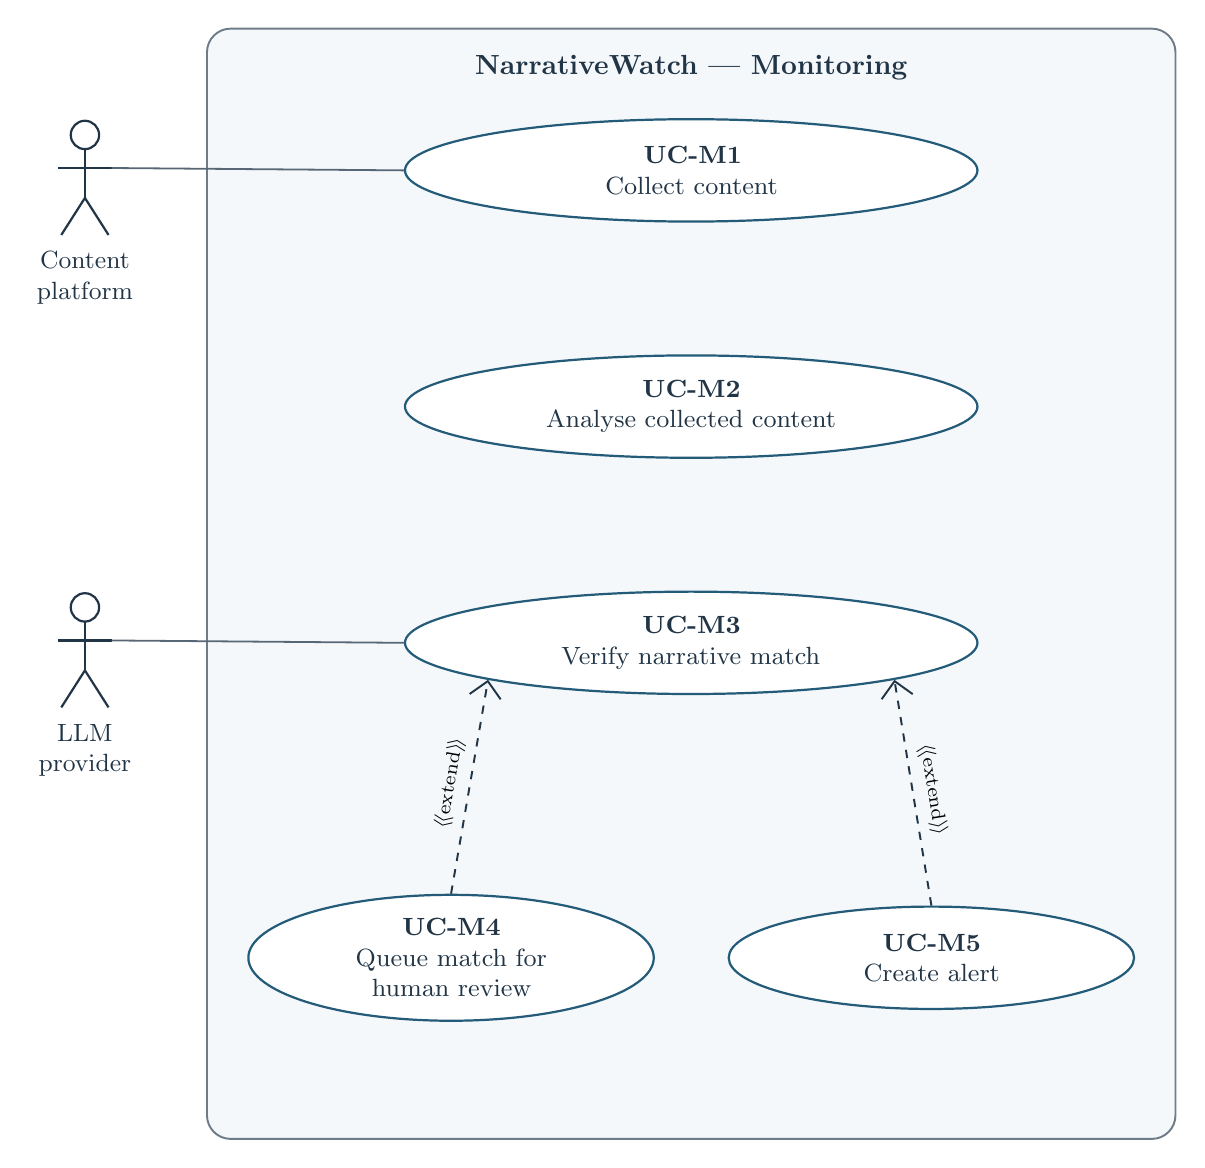
\begin{tikzpicture}[x=1cm,y=1cm,
  usecase/.append style={
    minimum width=7cm,
    text width=5cm
  }]

  \draw[boundary] (2.1,1.8) rectangle (14.4,-12.3);

  \node[font=\bfseries,text=ink] at (8.25,1.3)
    {NarrativeWatch --- Monitoring};

  \umlactor{platform}{.55}{0}
    {Content\\platform}

  \umlactor{provider}{.55}{-6}
    {LLM\\provider}

  \node[usecase] (collect) at (8.25,0)
    {\textbf{UC-M1}\\Collect content};

  \node[usecase] (analyse) at (8.25,-3)
    {\textbf{UC-M2}\\Analyse collected content};

  \node[usecase] (verify) at (8.25,-6)
    {\textbf{UC-M3}\\Verify narrative match};

  \node[usecase,minimum width=5cm,text width=3.5cm]
    (queue) at (5.2,-10)
    {\textbf{UC-M4}\\Queue match for\\human review};

  \node[usecase,minimum width=5cm,text width=3.5cm]
    (alert) at (11.3,-10)
    {\textbf{UC-M5}\\Create alert};

  \draw[association]
    (platform)--(collect.west);

  \draw[association]
    (provider)--(verify.west);

  \draw[dashed,-{Straight Barb[length=2mm]},
    draw=ink,line width=.7pt]
    (queue.north)--node[above,sloped,font=\scriptsize]
    {$\langle\!\langle$extend$\rangle\!\rangle$}
    (verify.south west);

  \draw[dashed,-{Straight Barb[length=2mm]},
    draw=ink,line width=.7pt]
    (alert.north)--node[above,sloped,font=\scriptsize]
    {$\langle\!\langle$extend$\rangle\!\rangle$}
    (verify.south east);

\end{tikzpicture}

\caption{Automatic content collection, narrative analysis
and verification.}
\label{fig:monitoring-use-cases}
\end{figure}

UC-M1 is handled by the Crawler Agent, UC-M2 by the
Analysis Agent and UC-M3 by the LLM Judge Module.
UC-M4 is triggered when a match requires human review,
while UC-M5 is triggered when the alert conditions are met.


\clearpage
\subsection{Analysis and Human Review}

These goals cover US-01--US-08 and US-12. Inspecting a result includes its
content, source, matched narrative, analysis score and Judge assessment.
Each narrative match is reviewed independently.

\begin{figure}[H]
\centering
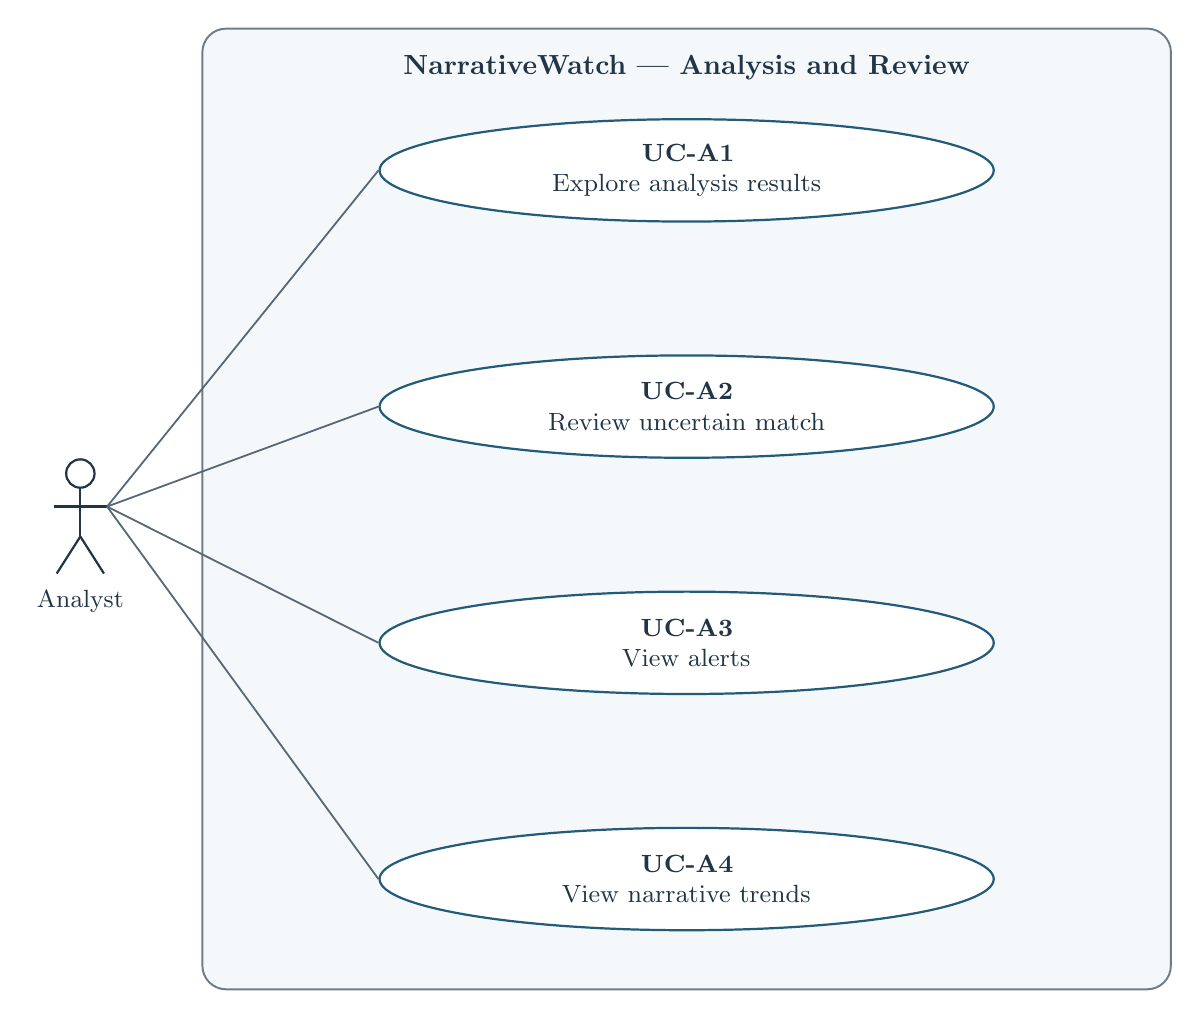
\begin{tikzpicture}[x=1cm,y=1cm,
  usecase/.append style={minimum width=7.8cm,text width=5.3cm}]
  \draw[boundary] (2.1,1.8) rectangle (14.4,-10.4);
  \node[font=\bfseries,text=ink] at (8.25,1.3)
    {NarrativeWatch --- Analysis and Review};
  \umlactor{analyst}{.55}{-4.3}{Analyst}

  \node[usecase] (results) at (8.25,0)
    {\textbf{UC-A1}\\Explore analysis results};
  \node[usecase] (review) at (8.25,-3)
    {\textbf{UC-A2}\\Review uncertain match};
  \node[usecase] (alerts) at (8.25,-6)
    {\textbf{UC-A3}\\View alerts};
  \node[usecase] (trends) at (8.25,-9)
    {\textbf{UC-A4}\\View narrative trends};

  \foreach \uc in {results,review,alerts,trends}
    \draw[association] (analyst)--(\uc.west);
\end{tikzpicture}
\caption{Main analyst goals, with detailed viewing operations grouped under UC-A1.}
\label{fig:analyst-use-cases}
\end{figure}

UC-A2 includes inspecting the selected match and saving the analyst's
confirmation or rejection as ground truth. These are steps of the review,
rather than separate use cases. From results or alerts, the analyst can
open the relevant match and start its review.

\clearpage
\subsection{Narrative Proposals and Peer Review}

Analysts can propose a narrative for a content item and review proposals
submitted by other analysts. A proposal's author cannot approve their
own proposal.

\begin{figure}[H]
\centering
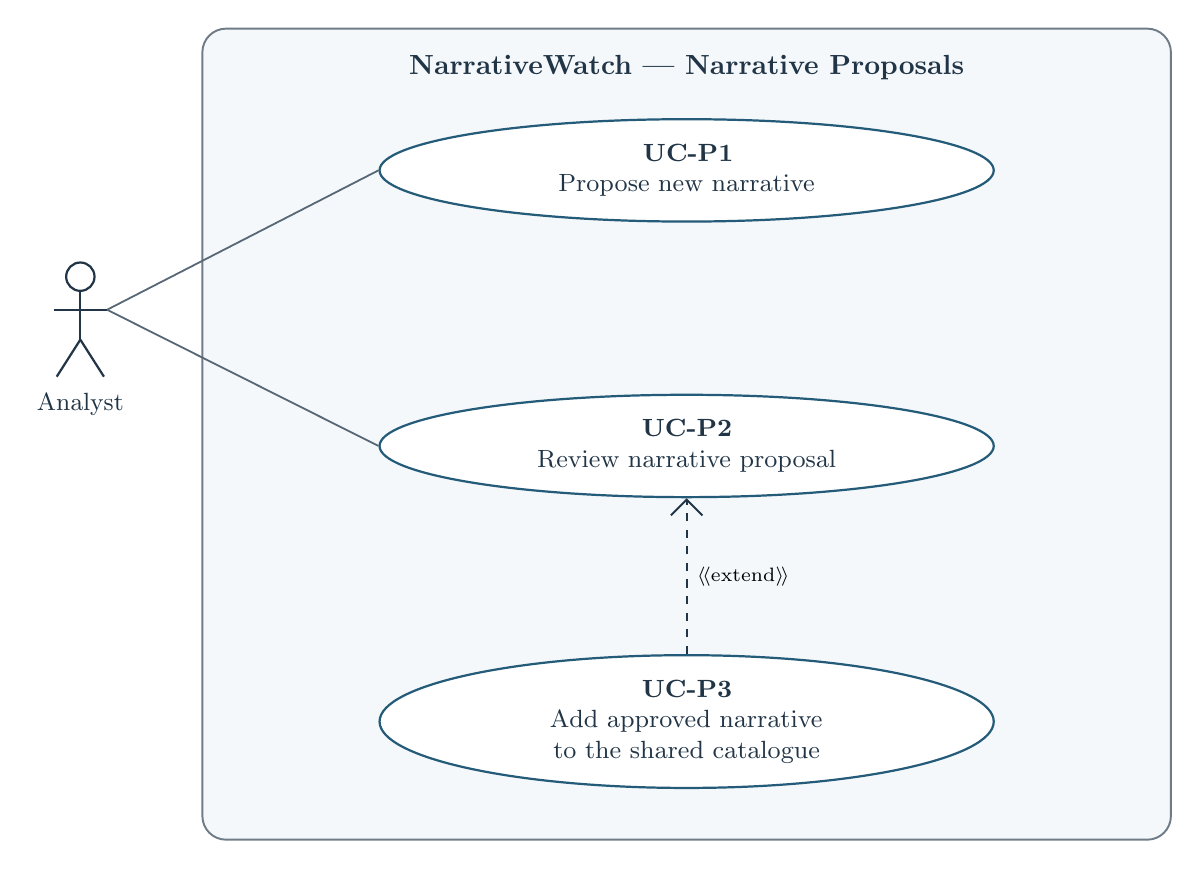
\begin{tikzpicture}[x=1cm,y=1cm,
  usecase/.append style={minimum width=7.8cm,text width=5.3cm}]
  \draw[boundary] (2.1,1.8) rectangle (14.4,-8.5);
  \node[font=\bfseries,text=ink] at (8.25,1.3)
    {NarrativeWatch --- Narrative Proposals};
  \umlactor{analyst}{.55}{-1.8}{Analyst}

  \node[usecase] (propose) at (8.25,0)
    {\textbf{UC-P1}\\Propose new narrative};
  \node[usecase] (peerreview) at (8.25,-3.5)
    {\textbf{UC-P2}\\Review narrative proposal};
  \node[usecase] (publish) at (8.25,-7)
    {\textbf{UC-P3}\\Add approved narrative\\to the shared catalogue};

  \draw[association] (analyst)--(propose.west);
  \draw[association] (analyst)--(peerreview.west);
  \draw[dashed,-{Straight Barb[length=2mm]},draw=ink,line width=.7pt]
    (publish.north)--node[right,font=\scriptsize]
    {$\langle\!\langle$extend$\rangle\!\rangle$}(peerreview.south);
\end{tikzpicture}
\caption{Proposing narratives, peer review and conditional catalogue inclusion.}
\label{fig:proposal-use-cases}
\end{figure}

The extension point in UC-P2 is after a review decision is recorded.
UC-P3 applies when the proposal satisfies the approval policy.
The required number of approvals and the decision policy remain to be
specified. Proposals can be submitted independently of a particular
uncertain-match review.

\clearpage
\subsection{Administration}


The administration use cases cover US-13--US-17.
They include managing monitored sources, managing known
FIMI narratives and viewing reviewer activity.

\begin{figure}[H]
\centering
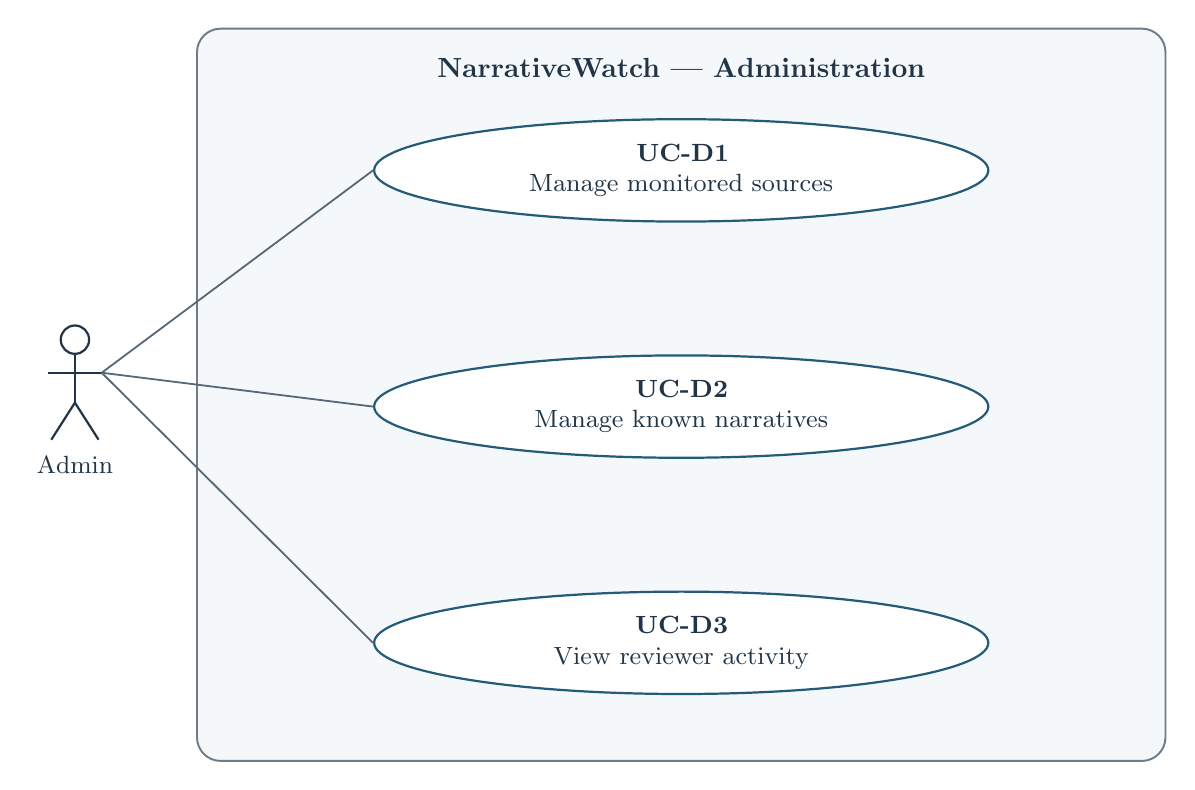
\begin{tikzpicture}[x=1cm,y=1cm,
  usecase/.append style={minimum width=7.8cm,text width=5.3cm}]
  \draw[boundary] (2.1,1.8) rectangle (14.4,-7.5);
  \node[font=\bfseries,text=ink] at (8.25,1.3)
    {NarrativeWatch --- Administration};
  \umlactor{admin}{.55}{-2.6}{Admin}

  \node[usecase] (sources) at (8.25,0)
    {\textbf{UC-D1}\\Manage monitored sources};
  \node[usecase] (narratives) at (8.25,-3)
    {\textbf{UC-D2}\\Manage known narratives};
  \node[usecase] (activity) at (8.25,-6)
    {\textbf{UC-D3}\\View reviewer activity};

  \foreach \uc in {sources,narratives,activity}
    \draw[association] (admin)--(\uc.west);
\end{tikzpicture}
\caption{Administration of monitoring resources and reviewer activity.}
\label{fig:admin-use-cases}
\end{figure}

UC-D3 shows the matches a reviewer confirmed or rejected, their proposed
narratives and their decisions on other analysts' proposals.
Login, logout and role-based permissions are described
in US-18--US-20.


\clearpage
\subsection{Communication Between Analysis and LLM Judge Modules}

The Analysis Module sends potential narrative matches
to the LLM Judge Module for verification.
The LLM Judge checks each match and returns a decision,
an explanation and a confidence score.

\begin{figure}[H]
\centering
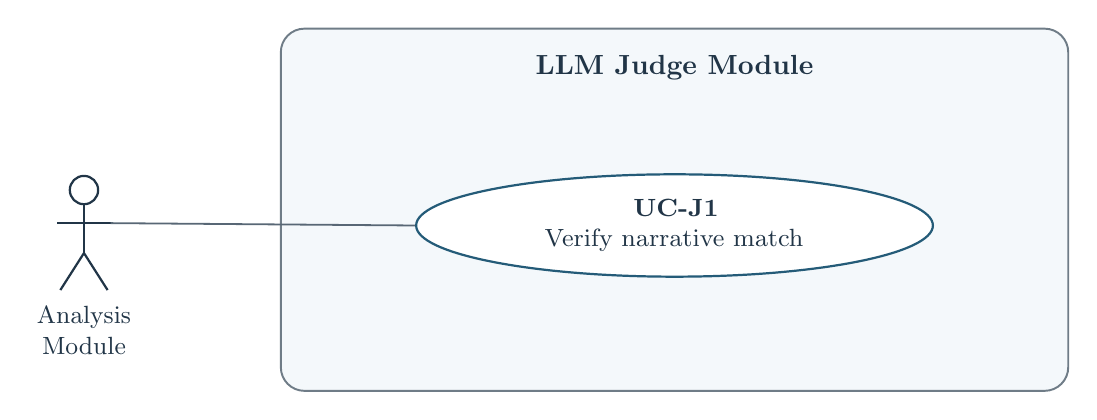
\begin{tikzpicture}[x=1cm,y=1cm,
  usecase/.append style={
    minimum width=6.2cm,
    text width=4.5cm
  }]

  \draw[boundary] (4,1) rectangle (14,-3.6);

  \node[font=\bfseries,text=ink] at (9,0.5)
    {LLM Judge Module};

  \umlactor{analysisactor}{1.5}{-1.5}
    {Analysis\\Module}

  \node[usecase] (verify) at (9,-1.5)
    {\textbf{UC-J1}\\Verify narrative match};

  \draw[association]
    (analysisactor)--(verify.west);

\end{tikzpicture}

\caption{Communication between the Analysis Module
and the LLM Judge Module.}
\label{fig:judge-module-use-case}
\end{figure}

The Analysis Module is a non-human actor in this diagram
because it interacts with the LLM Judge Module
through a service interface.

The service receives a candidate narrative match
and returns a verification result containing
a decision, explanation and confidence score.

UC-J1 describes the verification service of the LLM Judge
Module, which is also represented by UC-M3
in the monitoring diagram.


\clearpage


\begin{landscape}
\setlength{\intextsep}{6pt}
\captionsetup{skip=4pt}
\section{Class Diagrams}

The diagrams show domain classes that represent data and relationships and service classes that handle communication between modules.

\subsection{Domain Classes and Relationships}

Each match connects one content item with one narrative. Human review is
optional; narrative proposals have a separate review process.

\begin{figure}[H]
\centering
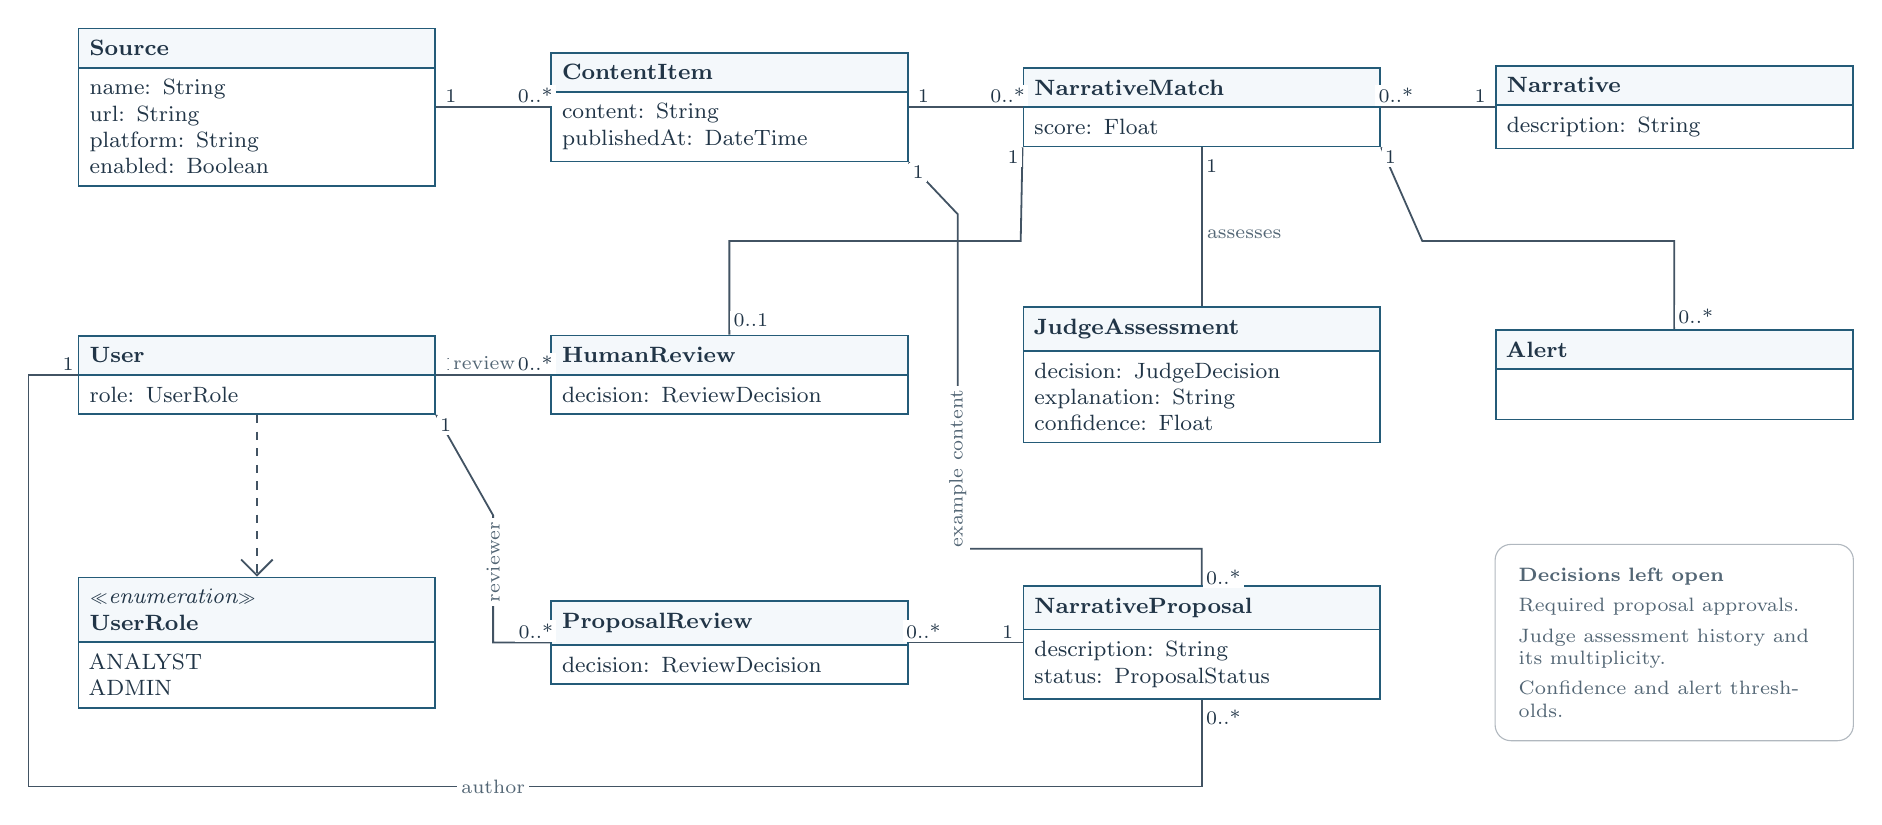
\begin{tikzpicture}[x=1cm,y=.85cm]
  \node[umlclass] (source) at (0,0)
    {\textbf{Source}\nodepart{second}
     name: String\\url: String\\platform: String\\enabled: Boolean};
  \node[umlclass] (content) at (6,0)
    {\textbf{ContentItem}\nodepart{second}
     content: String\\publishedAt: DateTime};
  \node[umlclass] (match) at (12,0)
    {\textbf{NarrativeMatch}\nodepart{second}score: Float};
  \node[umlclass] (narrative) at (18,0)
    {\textbf{Narrative}\nodepart{second}description: String};

  \node[umlclass] (user) at (0,-4)
    {\textbf{User}\nodepart{second}role: UserRole};
  \node[umlclass] (human) at (6,-4)
    {\textbf{HumanReview}\nodepart{second}decision: ReviewDecision};
  \node[umlclass] (judge) at (12,-4)
    {\textbf{JudgeAssessment}\nodepart{second}
     decision: JudgeDecision\\explanation: String\\confidence: Float};
  \node[umlclass] (alert) at (18,-4)
    {\textbf{Alert}\nodepart{second}\strut};

  \node[umlclass] (role) at (0,-8)
    {\textit{\guillemotleft enumeration\guillemotright}\\
     \textbf{UserRole}\nodepart{second}ANALYST\\ADMIN};
  \node[umlclass] (proposalreview) at (6,-8)
    {\textbf{ProposalReview}\nodepart{second}decision: ReviewDecision};
  \node[umlclass] (proposal) at (12,-8)
    {\textbf{NarrativeProposal}\nodepart{second}
     description: String\\status: ProposalStatus};
  \node[note,text width=3.95cm,font=\scriptsize] at (18,-8)
    {\textbf{Decisions left open}\\[3pt]
     Required proposal approvals.\\[3pt]
     Judge assessment history and its multiplicity.\\[3pt]
     Confidence and alert thresholds.};

  \draw[umlrelation] (source.east)--
    node[umlmultiplicity,above,pos=.13]{1}
    node[umlmultiplicity,above,pos=.87]{0..*}(content.west);
  \draw[umlrelation] (content.east)--
    node[umlmultiplicity,above,pos=.13]{1}
    node[umlmultiplicity,above,pos=.87]{0..*}(match.west);
  \draw[umlrelation] (match.east)--
    node[umlmultiplicity,above,pos=.13]{0..*}
    node[umlmultiplicity,above,pos=.87]{1}(narrative.west);

  \draw[umlrelation] (match.south)--
    node[umlmultiplicity,right,pos=.12]{1}
    node[umlcaption,right,pos=.55]{assesses}(judge.north);
  \draw[umlrelation] (match.south west)--(9.7,-2)--(6,-2)--
    node[umlmultiplicity,right,pos=.85]{0..1}(human.north);
  \node[umlmultiplicity,anchor=north east] at (match.south west) {1};
  \draw[umlrelation] (match.south east)--(14.8,-2)--(18,-2)--
    node[umlmultiplicity,right,pos=.85]{0..*}(alert.north);
  \node[umlmultiplicity,anchor=north west] at (match.south east) {1};

  \draw[umlrelation] (user.east)--
    node[umlmultiplicity,above,pos=.13]{1}
    node[umlcaption,above,pos=.5]{reviewer}
    node[umlmultiplicity,above,pos=.87]{0..*}(human.west);
  \draw[umldependency] (user.south)--(role.north);
  \draw[umlrelation] (user.south east)--(3,-6.1)--(3,-8)--
    node[umlmultiplicity,above,pos=.75]{0..*}(proposalreview.west);
  \node[umlmultiplicity,anchor=north west] at (user.south east) {1};
  \node[umlcaption,rotate=90] at (3,-6.8) {reviewer};

  \draw[umlrelation] (proposalreview.east)--
    node[umlmultiplicity,above,pos=.13]{0..*}
    node[umlmultiplicity,above,pos=.87]{1}(proposal.west);
  \draw[umlrelation] (content.south east)--(8.9,-1.6)--(8.9,-6.6)--
    (12,-6.6)--node[umlmultiplicity,right,pos=.8]{0..*}(proposal.north);
  \node[umlmultiplicity,anchor=north west] at (content.south east) {1};
  \node[umlcaption,rotate=90] at (8.9,-5.4) {example content};

  \draw[umlrelation] (user.west)--(-2.9,-4)--(-2.9,-10.15)--
    (12,-10.15)--node[umlmultiplicity,right,pos=.8]{0..*}(proposal.south);
  \node[umlmultiplicity,anchor=south east] at (user.west) {1};
  \node[umlcaption] at (3,-10.15) {author};
\end{tikzpicture}
\caption{Domain classes. Source and reviewer references are represented by
associations rather than duplicated attributes.}
\label{fig:domain-classes}
\end{figure}

{\small One source is a specific profile, channel or website. Review decisions
are confirmation or rejection. Only selected matches receive a HumanReview.
An approved NarrativeProposal is added to the shared Narrative catalogue;
its author cannot approve their own proposal.}

\clearpage
\subsection{Services and Communication}

Dashed arrows show which service uses another. Dashed arrows with a hollow
triangle show interface implementation. Parameters are abbreviated to keep
the diagram readable; \texttt{item} is a ContentItem and \texttt{match} is a
NarrativeMatch.

\begin{figure}[H]
\centering
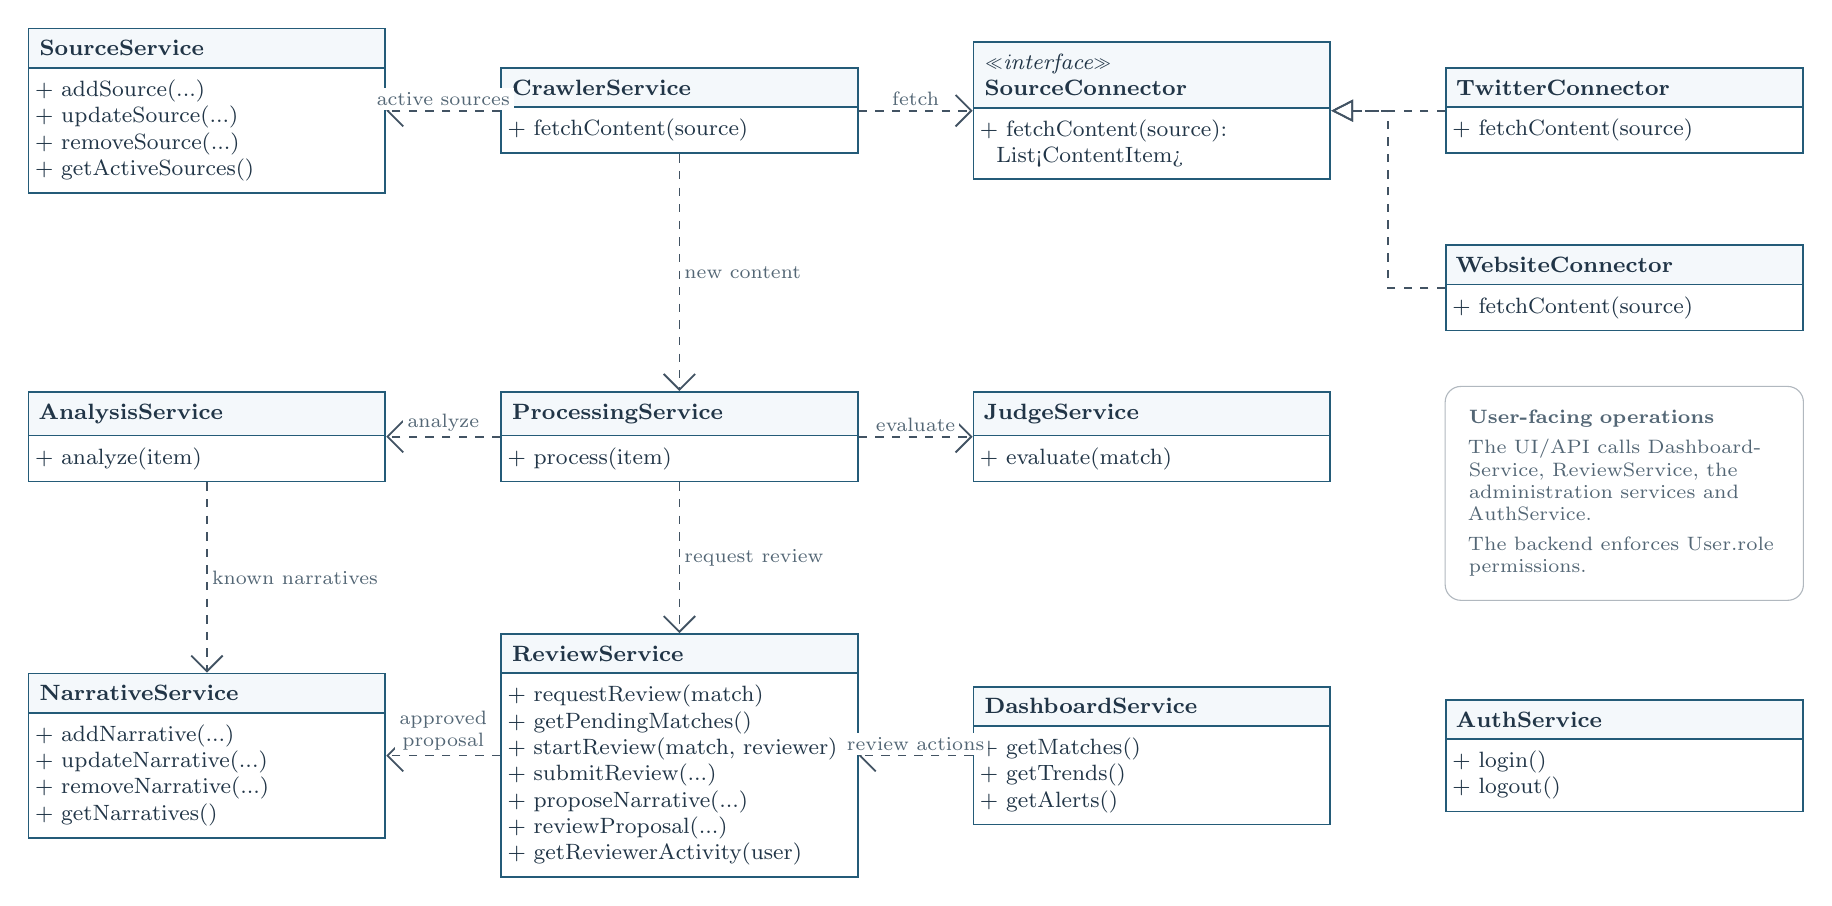
\begin{tikzpicture}[x=1cm,y=.90cm]
  \node[umlclass] (sourceservice) at (0,0)
    {\textbf{SourceService}\nodepart{second}
     + addSource(...)\\+ updateSource(...)\\+ removeSource(...)\\
     + getActiveSources()};
  \node[umlclass] (crawler) at (6,0)
    {\textbf{CrawlerService}\nodepart{second}+ fetchContent(source)};
  \node[umlclass] (connector) at (12,0)
    {\textit{\guillemotleft interface\guillemotright}\\
     \textbf{SourceConnector}\nodepart{second}
     + fetchContent(source):\\\hspace*{.5em}List<ContentItem>};
  \node[umlclass] (twitter) at (18,0)
    {\textbf{TwitterConnector}\nodepart{second}+ fetchContent(source)};
  \node[umlclass] (website) at (18,-2.5)
    {\textbf{WebsiteConnector}\nodepart{second}+ fetchContent(source)};

  \node[umlclass] (analysis) at (0,-4.6)
    {\textbf{AnalysisService}\nodepart{second}+ analyze(item)};
  \node[umlclass] (processing) at (6,-4.6)
    {\textbf{ProcessingService}\nodepart{second}+ process(item)};
  \node[umlclass] (judgeservice) at (12,-4.6)
    {\textbf{JudgeService}\nodepart{second}+ evaluate(match)};

  \node[umlclass] (narrativeservice) at (0,-9.1)
    {\textbf{NarrativeService}\nodepart{second}
     + addNarrative(...)\\+ updateNarrative(...)\\
     + removeNarrative(...)\\+ getNarratives()};
  \node[umlclass] (reviewservice) at (6,-9.1)
    {\textbf{ReviewService}\nodepart{second}
     + requestReview(match)\\+ getPendingMatches()\\
     + startReview(match, reviewer)\\+ submitReview(...)\\
     + proposeNarrative(...)\\+ reviewProposal(...)\\
     + getReviewerActivity(user)};
  \node[umlclass] (dashboard) at (12,-9.1)
    {\textbf{DashboardService}\nodepart{second}
     + getMatches()\\+ getTrends()\\+ getAlerts()};
  \node[umlclass] (auth) at (18,-9.1)
    {\textbf{AuthService}\nodepart{second}+ login()\\+ logout()};

  \draw[umldependency] (crawler.west)--
    node[umlcaption,above]{active sources}(sourceservice.east);
  \draw[umldependency] (crawler.east)--
    node[umlcaption,above]{fetch}(connector.west);
  \draw[umlrealisation] (twitter.west)--(connector.east);
  \draw[umlrealisation] (website.west)--(15,-2.5)--(15,0)--(connector.east);
  \draw[umldependency] (crawler.south)--
    node[umlcaption,right]{new content}(processing.north);
  \draw[umldependency] (processing.west)--
    node[umlcaption,above]{analyze}(analysis.east);
  \draw[umldependency] (processing.east)--
    node[umlcaption,above]{evaluate}(judgeservice.west);
  \draw[umldependency] (processing.south)--
    node[umlcaption,right]{request review}(reviewservice.north);
  \draw[umldependency] (analysis.south)--
    node[umlcaption,right]{known narratives}(narrativeservice.north);
  \draw[umldependency] (reviewservice.west)--
    node[umlcaption,above]{approved\\proposal}(narrativeservice.east);
  \draw[umldependency] (dashboard.west)--
    node[umlcaption,above]{review actions}(reviewservice.east);

  \node[note,text width=3.95cm,font=\scriptsize] at (18,-5.4)
    {\textbf{User-facing operations}\\[3pt]
     The UI/API calls DashboardService, ReviewService, the administration
     services and AuthService.\\[3pt]
     The backend enforces User.role permissions.};
\end{tikzpicture}
\caption{Service classes, their principal operations and dependencies.}
\label{fig:service-classes}
\end{figure}

{\small AnalysisService returns narrative matches; JudgeService returns a
JudgeAssessment for each match. ProcessingService creates alerts
and requests review according to the rules; both can apply
to the same match. ReviewService records decisions and narrative proposals.}

\end{landscape}


\end{document}
